\documentclass[a4paper,12pt]{article}

\usepackage{mystyle}

\graphicspath{ {images/} }


\newtheorem{theorem}{Теорема}[section]

\newtheorem*{problem}{Задача}

\theoremstyle{definition}
\newtheorem{definition}{Определение}[section]

\theoremstyle{remark}
\newtheorem*{example}{Пример}

\theoremstyle{remark}
\newtheorem*{remark}{Замечание}


\DeclareMathOperator{\Sp}{Sp}
\DeclareMathOperator{\Tr}{Tr}


\definecolor{cyanL}{RGB}{0, 204, 204}


\author{Алексеев Василий}
\title{Семинар 1}
\date{1 сентября 2020}



\begin{document}
  \maketitle
  \tableofcontents
  \thispagestyle{empty}
  
  \newpage
  
  \pagenumbering{arabic}

  % This line should be omitted when using XeLaTeX (only \section{...} etc. will be enough)
  %\addcontentsline{toc}{section}{Пролог}

  %\include{prologue}


  \section{Матрицы и определители $2$-го и $3$-го порядков}

  \subsection{Матрицы}

  Матрица $A$ размера $m \times n$:
  \[
    A = \begin{pmatrix}
      a_{11} & a_{12} & \ldots & a_{1n}\\
      a_{21} & a_{22} & \ldots & a_{2n}\\
      \vdots & \vdots & \ddots & \vdots\\
      a_{m1} & a_{m2} & \ldots & a_{mn}
    \end{pmatrix} \in \RR^{m \times n}
  \]
  
  
  \subsubsection{Операции с матрицами}
  
  \begin{definition}[Сложение матриц]
    Пусть $A, B \in \RR^{n \times n}$.
    Суммой $A \hm+ B$ называется матрица $C \hm\in \RR^{n \times n}$, такая что
    $c_{ij} \hm= a_{ij} + b_{ij}$, $i, j \hm= 1, \ldots, n$.
  \end{definition}
  
  \begin{definition}[Умножение матрицы на число]
    Пусть $A \in \RR^{n \times n}, \alpha \in \RR$.
    Произведением матрицы $A$ на число $\alpha$ называется матрица $C$, такая что
    $c_{ij} \hm= \alpha \cdot a_{ij}$, $i, j \hm= 1, \ldots, n$.
  \end{definition}
  
  \begin{remark}
    Матрицы $\RR^{n \times n}$ с введённой операцией сложения и умножения на числа из $\RR$ образуют линейное пространство\footnote{\href{https://en.wikipedia.org/wiki/Vector\_space}{wikipedia.org/wiki/Vector\_space}}:
    \begin{enumerate}
      \item $A + B = B + A$, $\forall A, B \in \RR^{n \times n}$ (коммутативность сложения).
      \item $A + (B + C) = (A + B) + C$, $\forall A, B, C \in \RR^{n \times n}$ (ассоциативность сложения).
      \item $\exists 0_{n\times n} \in \RR^{n \times n}: 0_{n\times n} + A = A$, $\forall A \hm\in \RR^{n \times n}$.
      \item $\forall A \in \RR^{n \times n} \exists -A \in \RR^{n \times n}: A + (-A) = 0_{n\times n}$.
      \item $\alpha (\beta A) = (\alpha \beta) A$, $\forall \alpha, \beta \in \RR$, $\forall A \hm\in \RR^{n \times n}$ (ассоциативность умножения на скаляр).
      \item $1 \cdot A = A$, $\forall A \in \RR^{n \times n}$.
      \item $(\alpha + \beta) A = \alpha A + \beta A$, $\forall \alpha, \beta \hm\in \RR$, $A \hm\in \RR^{n \times n}$ (дистрибутивность умножения матрицы на число относительно сложения чисел).
      \item $\alpha (A + B) = \alpha A + \alpha B$, $\forall \alpha \hm\in \RR$, $A, B \hm\in \RR^{n \times n}$ (дистрибутивность умножения матрицы на число относительно сложения матриц).
    \end{enumerate}
  \end{remark}
  
  \begin{definition}[Умножение матриц]
    Пусть $A \hm\in \RR^{m \times p}$, $B \hm\in \RR^{p \times n}$.
    Тогда матрица $C$ называется произведением матриц $A$ и $B$, если
    \[
      c_{ij} = \sum_{k = 1}^p a_{ik} b_{kj}
    \]
    и обозначается $C \hm= AB$.
  \end{definition}

  \begin{figure}[h]
    \centering
    
    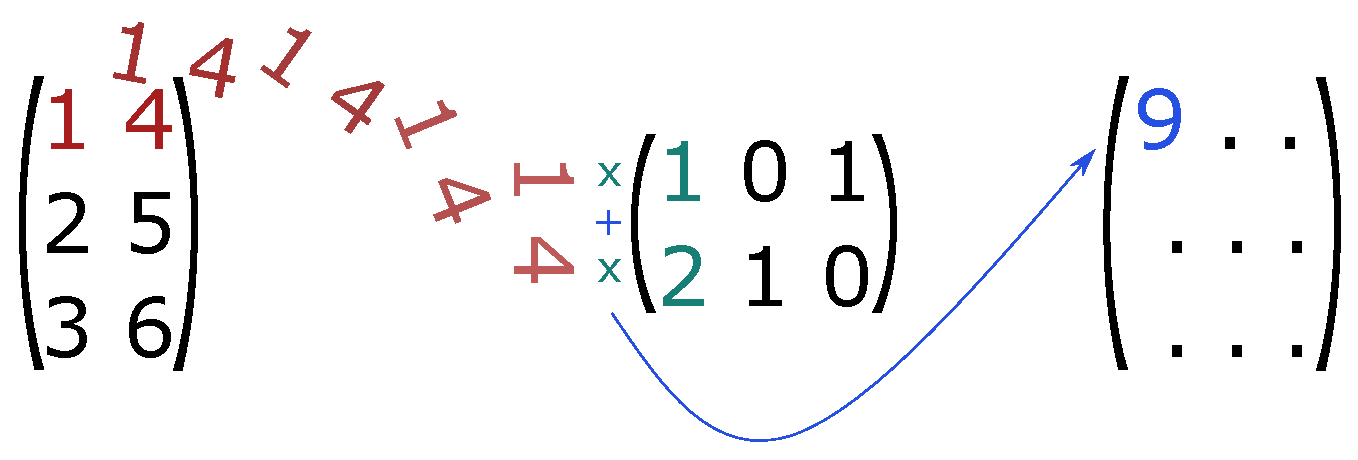
\includegraphics[width=0.5\columnwidth]{matrix-multiplication}
    
    \caption{Иллюстрация умножения матриц.}
    \label{fig:matrix-multiplication}
  \end{figure}
  
  \begin{problem}[15.5(7)]
    \[
      \left\{
        \begin{aligned}
          &A_{110} A_{12} = \?\\
          &A_{110} = \begin{pmatrix}
            3 & 1\\
            2 & 1\\
            1 & 0
          \end{pmatrix}\\
          &A_{12} = \begin{pmatrix}
            1 & 1\\
            1 & 1
          \end{pmatrix}
        \end{aligned}
      \right.
    \]
  \end{problem}
  
  \emph{Решение}
  
  \[
    A_{110} A_{12}
    = \begin{pmatrix}
      3 \cdot 1 + 1 \cdot 1 & 3 \cdot 1 + 1 \cdot 1\\
      2 \cdot 1 + 1 \cdot 1 & 2 \cdot 1 + 1 \cdot 1\\
      1 \cdot 1 + 0 \cdot 1 & 1 \cdot 1 + 0 \cdot 1
    \end{pmatrix}
    = \begin{pmatrix}
      4 & 4\\
      3 & 3\\
      1 & 1
    \end{pmatrix}
  \]
  
  \qed
  
  \begin{definition}[Транспонирование матрицы]
    Пусть $A \in \RR^{n \times n}$.
    Тогда транспонированной по отношению к матрице $A$ матрицей называется такая матрица $С$, что
    $c_{ij} \hm= a_{ji}$.
    Транспонированная матрица обозначается $A^T$.
  \end{definition}
  
  \begin{definition}[След матрицы]
    Следом матрицы $A \in \RR^{n \times n}$ называется сумма элементов, находящихся на главной диагонали $\{a_{ij} \hm\mid i = j, i = 0, \ldots, n\}$:
    \[
      \Sp A \equiv \Tr A \equiv \sum_{i = 1}^n a_{ii}
    \]
  \end{definition}


  \subsection{Определитель матрицы}
  
  \begin{example}
    Определитель второго порядка:
    \[
      \begin{vmatrix}
        a & b\\
        c & d
      \end{vmatrix} = ad - cb
    \]
  \end{example}

  \begin{example}
    Определитель третьего порядка:
    \[
      \begin{vmatrix}
        a_1 & b_1 & c_1\\
        a_2 & b_2 & c_2\\
        a_3 & b_3 & c_3
      \end{vmatrix} =
        a_1 \cdot \begin{vmatrix}b_2 & c_2\\b_3 & c_3\end{vmatrix}
        - b_1 \cdot \begin{vmatrix}a_2 & c_2\\a_3 & c_3\end{vmatrix}
        + c_1 \cdot \begin{vmatrix}a_2 & b_2\\a_3 & b_3\end{vmatrix}
    \]
  \end{example}
  
  \begin{problem}[14.7(3)]
    \[
      \left\{
        \begin{aligned}
          &\det A_{202} = \?\\
          &A_{202} = \begin{pmatrix}
            1 & 2 & 2\\
            2 & 1 & -2\\
            2 & -2 & 1
          \end{pmatrix}
        \end{aligned}
      \right.
    \]
  \end{problem}
  
  \emph{Решение}
  
  \[
    \det A_{202}
    = 1 \cdot \Bigl(1 \cdot 1 - (-2) \cdot (-2)\Bigr)
      \textcolor{cyanL}{-} 2 \cdot \Bigl(2 \cdot 1 - 2 \cdot (-2)\Bigr)
      + 2 \cdot \Bigl(2 \cdot (-2) - 2 \cdot 1\Bigr)
    = -3 - 12 - 12
    = -27
  \]
  
  \qed
  
  \begin{example}
    Определитель единичной матрицы:
    \[
      \det E = 1^n = 1
    \]
  \end{example}

  \begin{definition}[Вырожденная матрица]
    Матрица $A$ называется вырожденной, если $\det A \hm= 0$.
    В противном случае матрица $A$ называется невырожденной.
  \end{definition}
  
  \begin{theorem}[Формула полного разложения определителя]\label{theor:complete-expansion}
    Пусть $A \in \RR^{n \times n}$.
    Тогда определитель $\det A$ матрицы равен
    \[
      \det A \equiv |A| \equiv \sum_{(i_1, \ldots, i_n)} (-1)^{N(i_1, \ldots, i_n)} a_{1 i_1} \ldots a_{n i_n}
    \]
  \end{theorem}
  
  \begin{theorem}
    Определитель транспонированной матрицы
    \[
      \det A^T = \det A
    \]
  \end{theorem}
  
  \begin{theorem}
    Определитель произведения двух квадратных матриц:
    \[
      \det (AB) = \det A \cdot \det B
    \]
  \end{theorem}
  
  
  \subsubsection{Свойства определителя}
  
  \begin{theorem}[Линейность по столбцу (строке)]
    \[
      \det (\bds a_1, \ldots, \underbrace{\bds p + \bds q}_{\bds a_i}, \ldots, \bds a_n)
      = \det (\bds a_1, \ldots, \bds p, \ldots, \bds a_n)
      + \det (\bds a_1, \ldots, \bds q, \ldots, \bds a_n)
    \]
    \[
      \det (\bds a_1, \ldots, \underbrace{\alpha \bds p}_{\bds a_i}, \ldots, \bds a_n)
      = \alpha \det (\bds a_1, \ldots, \bds p, \ldots, \bds a_n)
    \]
  \end{theorem}
  
  \begin{theorem}
    При перестановке двух (строк или столбцов) матрицы её определитель меняет знак.
    \[
      \det (\bds a_1, \ldots, \bds a_i, \ldots, \bds a_j, \ldots, \bds a_n)
      = -\det (\bds a_1, \ldots, \bds a_j, \ldots, \bds a_i, \ldots, \bds a_n)
    \]
  \end{theorem}
  
  \begin{theorem}
    Если две строки (два столбца) матрицы совпадают, то её определитель равен нулю.
    \[
      \det (\bds a_1, \ldots, \bds p, \ldots, \bds p, \ldots, \bds a_n) = 0
    \]
  \end{theorem}
  
  Свойства можно доказать как следствия теоремы \ref{theor:complete-expansion}.
  

  \section{Системы линейныx уравнений. Правило Крамера}
  
  Система $m$ линейных уравнений с $n$ неизвестными:
  \[
    \renewcommand{\arraycolsep}{2pt}
    \left\{
      \begin{array}{lcl}
        a_{11} x_1 + \ldots + a_{1n} x_n & = & b_1\\
        \hdotsfor{3}\\
        a_{m1} x_1 + \ldots + a_{mn} x_n & = & b_n
      \end{array}
    \right.
  \]
  
  В матричном виде:
  \[
    \begin{pmatrix}
      a_{11} & \ldots & a_{1n}\\
      \vdots & \ddots & \vdots\\
      a_{m1} & \ldots & a_{mn}
    \end{pmatrix}
    \begin{pmatrix}
      x_1\\
      \vdots\\
      x_n
    \end{pmatrix}
    =
    \begin{pmatrix}
      b_1\\
      \vdots\\
      b_n
    \end{pmatrix}
  \]
  
  Или так:
  \[
    A \bds x = \bds b
  \]
  
  \begin{definition}[Решение системы]
    \[
      \{\bds x \in \RR^N \mid A \bds x = \bds b\}
    \]
  \end{definition}
  
  \begin{definition}
    Система называется совместной, если она имеет хотя бы одно решение, и несовместной, если у неё нет решений.
  \end{definition}
  
  \begin{definition}
    Говорят, что система $B$ следует из системы $A$, если множество решений $B$ содержит множество решений $A$ \ref{fig:a-and-b-sets}.
  \end{definition}
  
  \begin{figure}[h]
    \centering
    
    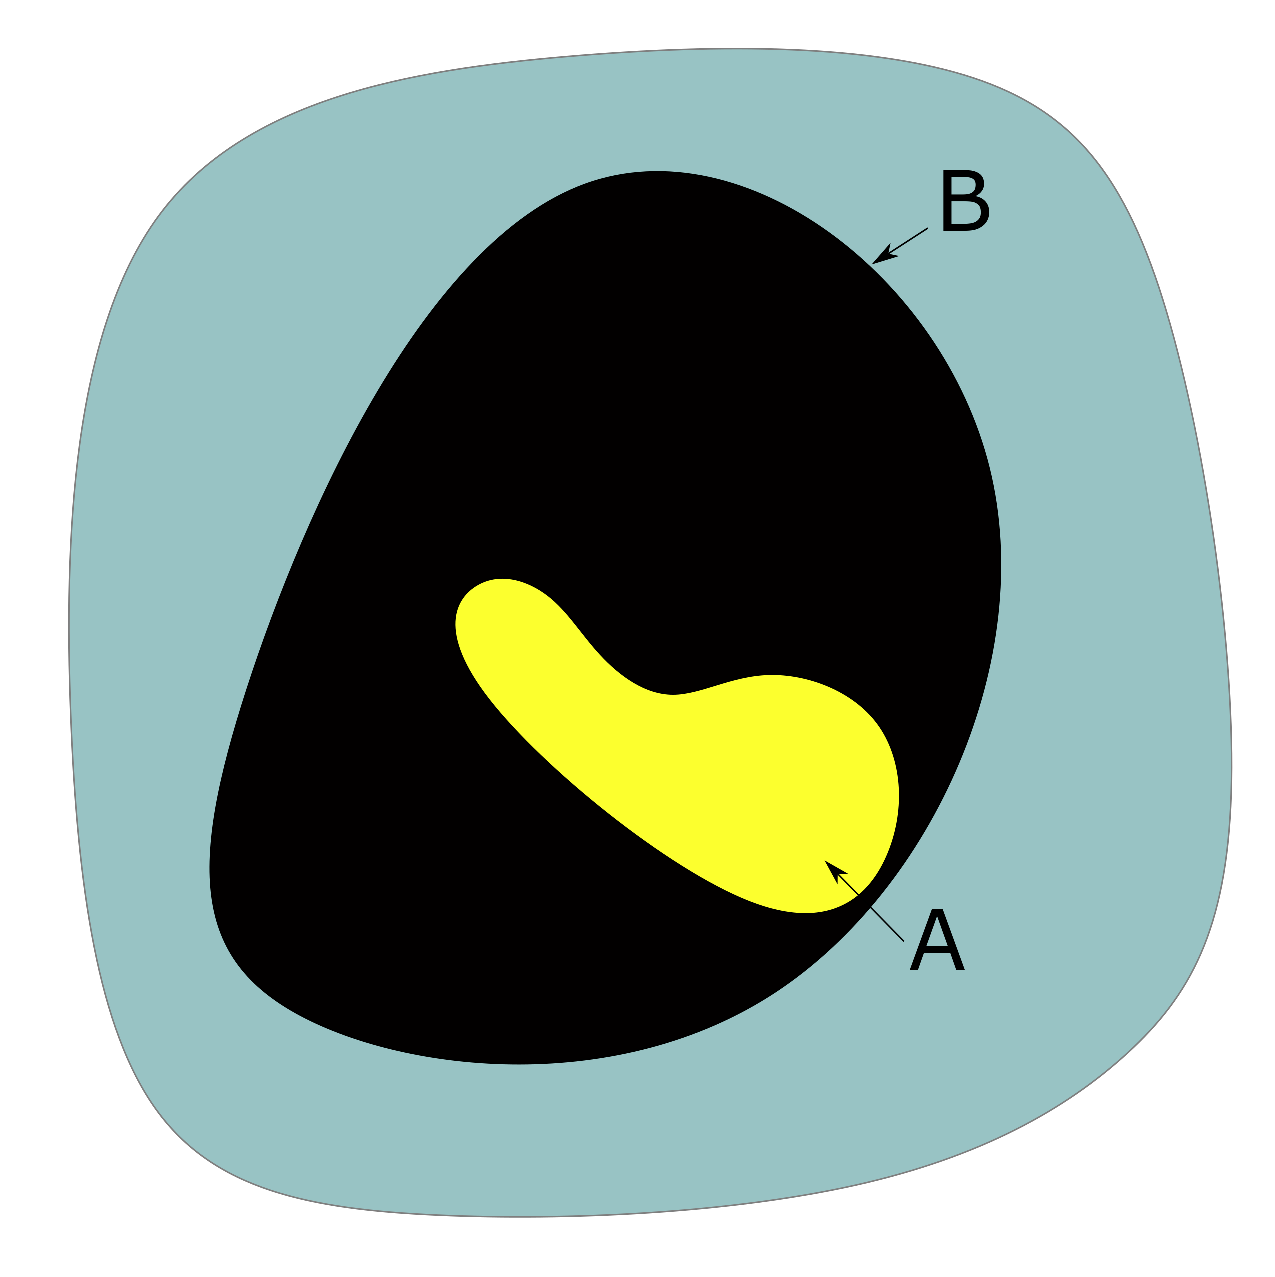
\includegraphics[width=0.5\columnwidth]{a-and-b-sets}
    
    \caption{Множество решений $A$ содержится во множестве решений $B$.}
    \label{fig:a-and-b-sets}
  \end{figure}
  
  \begin{theorem}
    Пусть число уравнений в системе $m$ равно числу неизвестных $n$.
    Тогда если $\det A \hm{\not=} 0$, то система $A \bds x \hm= \bds b$ имеет решение, и притом только одно.
  \end{theorem}
  
  \begin{theorem}[Правило Крамера]
    Пусть число уравнений в системе $m$ равно числу неизвестных $n$.
    Тогда если $\det A \hm{\not=} 0$, то
    \[
      \left\{
        \begin{aligned}
          &x_i = \frac{\Delta_i}{\Delta}\\
          &\Delta \equiv \det A\\
          &\Delta_i \equiv \det (\bds a_1, \ldots, \bds a_{i - 1}, \bds b, \bds a_{i + 1}, \ldots, \bds a_n)
        \end{aligned}
      \right.
    \]
  \end{theorem}
  
  \begin{problem}[17.2(4)]
    \[
      \left\{
        \begin{aligned}
          &A \bds x = \bds b\\
          &A = \begin{pmatrix}
            1 & -3 & -1\\
            -2 & 7 & 2\\
            3 & 2 & -4
          \end{pmatrix}\\
          &\bds b = \begin{pmatrix}
            -4\\ 10\\ 9
          \end{pmatrix}
        \end{aligned}
      \right.
    \]
  \end{problem}
  
  \emph{Решение}
  
  \[
    \Delta = \det \begin{pmatrix}
      1 & -3 & -1\\
      -2 & 7 & 2\\
      3 & 2 & -4
    \end{pmatrix} = -1
  \]
  \[
    \Delta_1 = \det \begin{pmatrix}
      -4 & -3 & -1\\
      10 & 7 & 2\\
      9 & 2 & -4
    \end{pmatrix} = -3 \Rightarrow x_1 = \frac{\Delta_1}{\Delta} = \frac{-3}{-1} = 3
  \]
  \[
    \Delta_2 = \det \begin{pmatrix}
      1 & -4 & -1\\
      -2 & 10 & 2\\
      3 & 9 & -4
    \end{pmatrix} = -2 \Rightarrow x_2 = \frac{\Delta_2}{\Delta} = \frac{-2}{-1} = 2
  \]
  \[
    \Delta_3 = \det \begin{pmatrix}
      1 & -3 & -4\\
      -2 & 7 & 10\\
      3 & 2 & 9
    \end{pmatrix} = -1 \Rightarrow x_3 = \frac{\Delta_3}{\Delta} = \frac{-1}{-1} = 1
  \]
  \[
    \bds x = \begin{pmatrix}
      3\\ 2\\ 1
    \end{pmatrix}
  \]
  
  \qed
  
\end{document}